\section{Full joint mixed-integer benchmark}\label{sec:joint}
\label{sec:breadth}
A frozen public synthetic grid crosses 24/72/144 nominal optional instruments, 2/6 discretionary tickets, disjoint/overlapping groups and tight/wide cash and group bands. Seed 111001 supplies 24 paired instances; seed 112001 supplies two eight-instrument controls. The generator retains two forced exits, a 50 NAV bp minimum ticket and a 25 NAV bp holding floor. The V2 heuristic and rules remain frozen. This paired rerun corrects the MIQP reference's native feasibility setting and quadratic-cone scaling after this grid exposed a false optimal termination. It is a numerical regression comparison, not an untouched validation of the corrected reference. Factorial variants share random draws and are not independent market replications.

Each joint MIQP optimises all admissible states and sizes simultaneously in the same prepared CORRIDOR domain. MIP-B starts from the common prepared incumbent; MIP-V receives only V2's audited proposal. Suffixes denote 10/60/600-second wrapper allowances. Every call starts afresh: incumbents never pass between budgets. Native calls use one thread, seed zero and the same $10^{-4}$ relative-gap setting; native integer feasibility is $10^{-9}$. Budget and start orders alternate deterministically. The mathematical MIQP is solved in an algebraically equivalent, balanced conic representation.

All 24 broad cases were attempted; 24 prepared. Effective optional candidates range from 20 to 41. Table~\ref{tab:joint} reports audited outputs over the full expected denominator. Tracking-error means use audited outputs; time summaries include every attempted arm. End-to-end (E2E) adds preparation to every arm and V2 generation to each MIP-V call.

\begin{table}[htbp]\centering\small\setlength{\tabcolsep}{4pt}
\caption{Full joint optimisation versus V2. TE is annual bp; E2E time is seconds.}\label{tab:joint}
\begin{tabular}{lrrrrr}\toprule
Arm & Audited & Mean TE & Median E2E & 95th pct. & V2 worse\\\midrule
V2 & 24/24 & 132.960 & 1.559 & 6.849 & --\\
MIP-B10 & 24/24 & 132.960 & 0.171 & 0.551 & 0\\
MIP-V10 & 24/24 & 132.960 & 1.892 & 7.202 & 0\\
MIP-B60 & 24/24 & 132.960 & 0.166 & 0.551 & 0\\
MIP-V60 & 24/24 & 132.960 & 1.895 & 7.184 & 0\\
MIP-B600 & 24/24 & 132.960 & 0.165 & 0.555 & 0\\
MIP-V600 & 24/24 & 132.960 & 1.889 & 7.219 & 0\\
\bottomrule\end{tabular}\end{table}

\begin{figure}[htbp]\centering
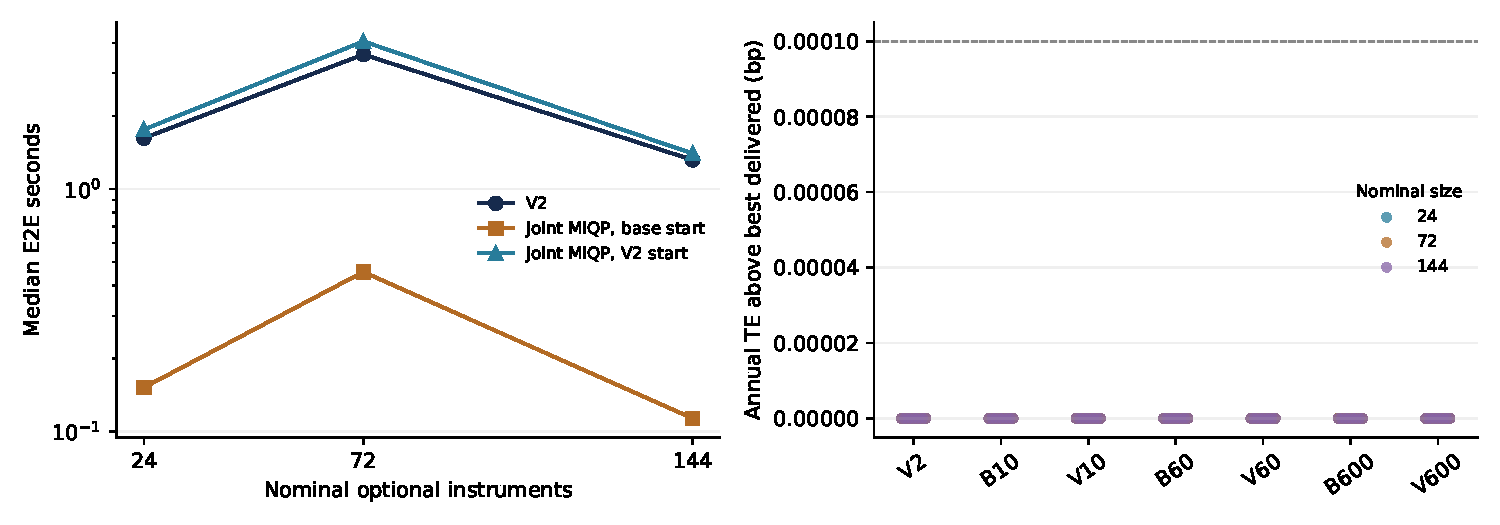
\includegraphics[width=\linewidth]{figures/joint_comparison.pdf}
\caption{Left: median E2E computation at the 600-second wrapper allowance, including preparation and V2 start generation. Right: each audited outcome above the best delivered TE on that case; this pooled reporting reference is never supplied as a start. Points identify nominal optional-universe size; the dashed line is the unchanged descriptive equality band.}\label{fig:joint}
\end{figure}

V2 exceeds the best audited delivery by more than the $10^{-4}$ bp descriptive band on 0/24 cases; its largest delivered gap is 0.000000 bp. A worse time-limited MIP delivery does not imply a worse mathematical optimum. A tie with MIP-V may simply retain V2's supplied incumbent. All native/retained/refined sources, first native audited feasibility times, failed outputs and allowance overruns are preserved in the numerical summary.

Changing the allowance changes delivered TE above the descriptive band on 0 common-base and 0 V2-started cases. These allowances are upper limits, not enforced run durations. At 600 seconds, V2 has lower TE than the common-base delivery on 0/24 cases and ties on 24/24; its largest advantage is 0.000000 bp. MIP-V600 retains the supplied V2 start on 12 cases.

Across all six MIQP arms, 0 native bounds exceed a better audited cross-arm objective at the unchanged $10^{-12}$ variance comparison scale. Raw bounds and statuses are retained, not clipped to the incumbent. Consistency with delivered witnesses is necessary but does not independently certify the native branch-and-bound result.

Separate conservative relaxation bounds close within the descriptive band on 0/24 cases. Their median/maximum best-delivery gaps are 4.153/20.025 bp; there are 0 upper/lower inconsistencies. Native optimal status and solver-reported MIP gaps remain diagnostics, not independent global certificates.

Independent full-weight QP enumeration covers 74 supports across 2 tiny cases; 2 enumerations are complete and 0 supports remain unresolved. The maximum absolute delivered difference across all tiny arms is 3.55e-09 bp. These are floating-point numerical references, not exact-arithmetic proofs.

The earlier development, holdout and search-ablation records remain in the replication package. This rerun changes only the reference's internal numerical setting, conic scaling and diagnostic checks, preserving the heuristic and production policy. Computational cost is measured rather than assumed: the experiment establishes neither a universal speed advantage nor realised investment performance.
